% \documentclass[handout]{beamer}
\documentclass[presentation]{beamer}
\usecolortheme{duxing}
\usefonttheme{duxing}
\useinnertheme{duxing}
 
\usepackage[utf8]{inputenc}
\usepackage[UKenglish]{babel}
\usepackage{booktabs}
\usepackage{caption}
\usepackage{subcaption}
\usepackage{graphicx}
\usepackage{amsmath, bm}
\usepackage{amsfonts}
\usepackage{amssymb}

\institute{
\includegraphics[height=0.7cm]{sysu_logo.png}
\includegraphics[height=0.7cm]{duxing_logo.png}}

\title{Application of Deep Learning}


\author{Tao Huang}

\date{}


\begin{document}
 
\frame{\titlepage}

\section{Neural Networks}

\begin{frame}
    \frametitle{Universal approximation theorem}

    Let $\varphi :\mathbb {R} \to \mathbb {R}$ be a nonconstant, bounded, and continuous function (called the activation function). Let $I_m$ denote the m-dimensional unit hypercube $[0,1]^{m}$. The space of real-valued continuous functions on $I_m$ is denoted by $C(I_{m})$. Then, given any $\varepsilon >0$ and any function $f\in C(I_{m})$, there exist an integer $N$, real constants $v_{i},b_{i}\in {\mathbb  {R}}$ and real vectors $w_{i}\in \mathbb {R} ^{m}$ for $i=1,\ldots ,N$, such that we may define:
    \begin{equation}
        F(x)=\sum _{{i=1}}^{{N}}v_{i}\varphi \left(w_{i}^{T}x+b_{i}\right)
    \end{equation}
    as an approximate realization of the function $f$; that is,
    \begin{equation}
        | F( x ) - f ( x ) | < \varepsilon
    \end{equation}
    for all $x\in I_{m}$.

\end{frame}

\begin{frame}
    \frametitle{Classification and Regression}

    Classification is about predicting a \textbf{label} and regression is about predicting a \textbf{quantity}.

\end{frame}

\section{Computer Vision}

\begin{frame}[allowframebreaks]
    \frametitle{Image Classification}

    \begin{figure}
        \centering
        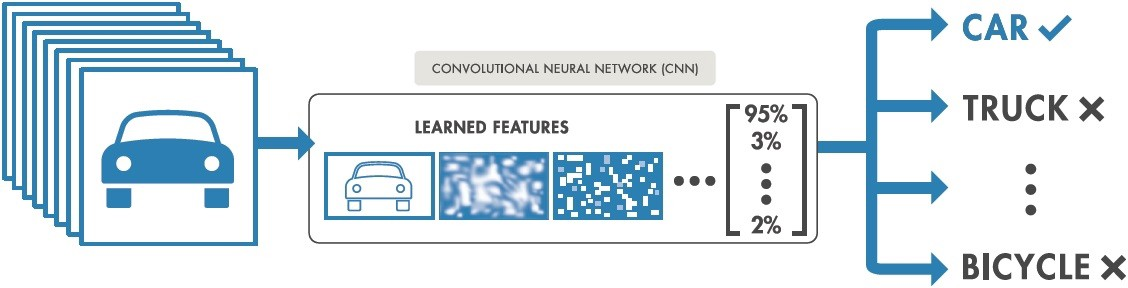
\includegraphics[width=0.95\linewidth]{1.jpeg}
        \caption{}
        Source : MathWorks \url{https://goo.gl/zondfq}
    \end{figure}

    \begin{figure}
        \centering
        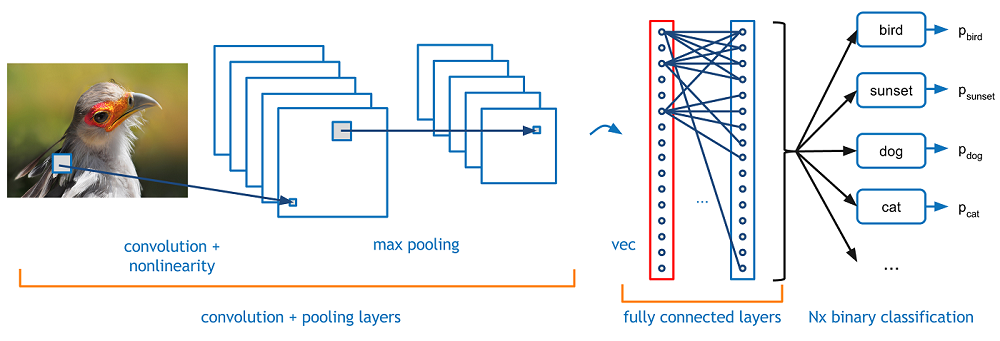
\includegraphics[width=0.95\linewidth]{1_1.png}
        \caption{Convolutional neural network}
    \end{figure}

    \begin{figure}
        \centering
        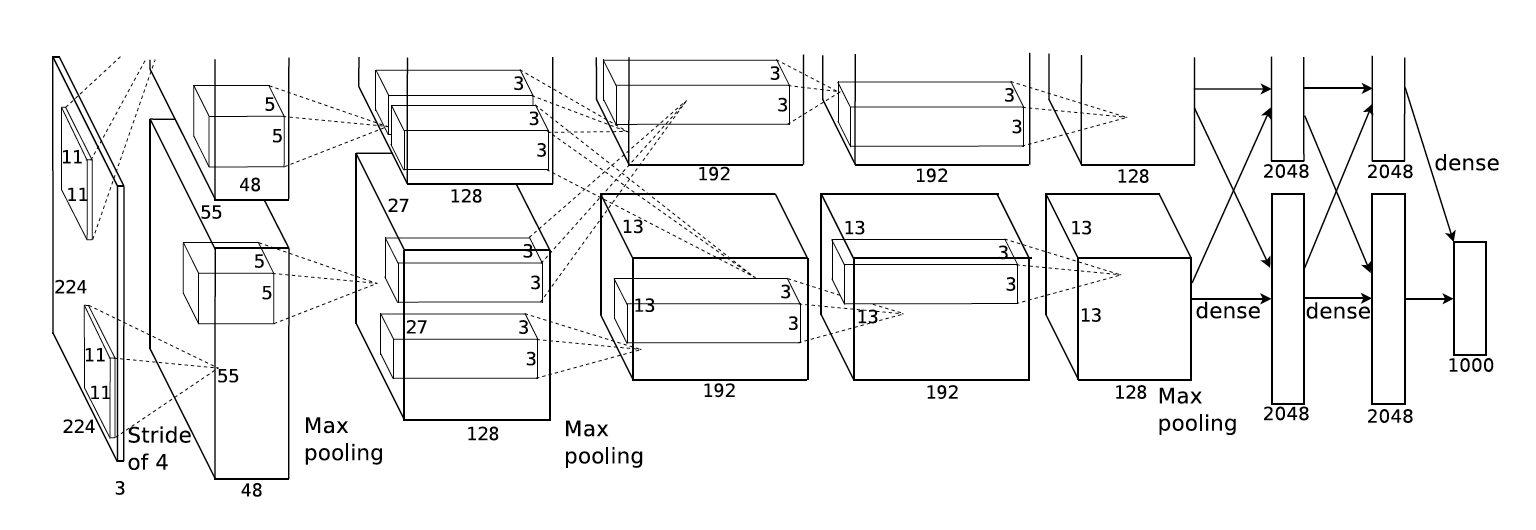
\includegraphics[width=0.95\linewidth]{1_2.png}
        \caption{AlexNet}
    \end{figure}

    \begin{figure}
        \centering
        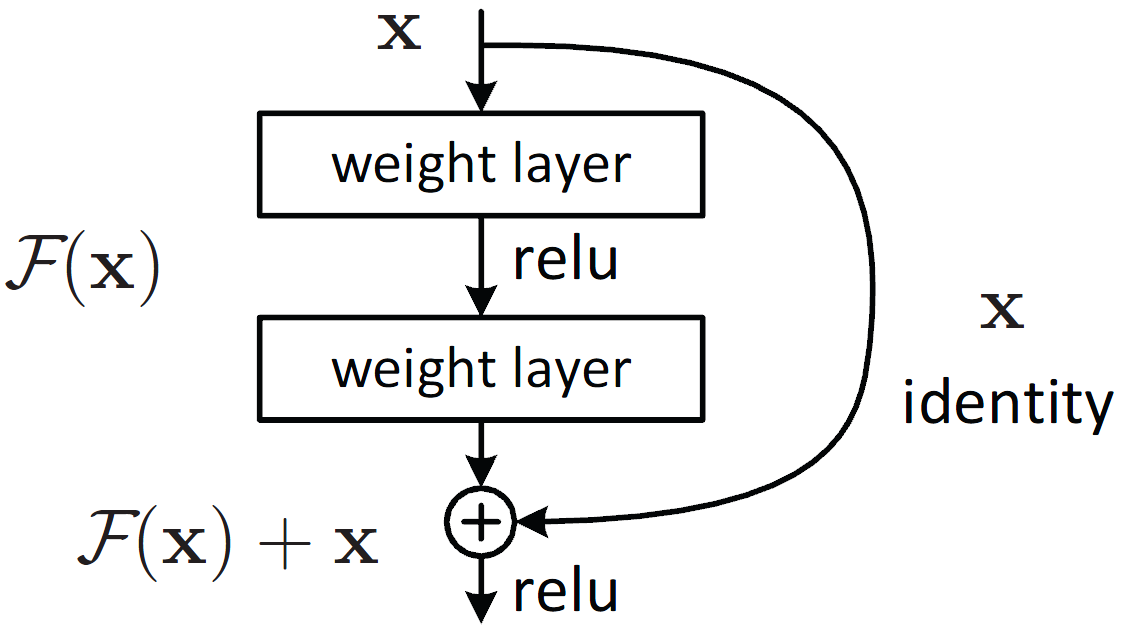
\includegraphics[width=0.8\linewidth]{1_3.png}
        \caption{ResNet}
    \end{figure}

    \begin{figure}
        \centering
        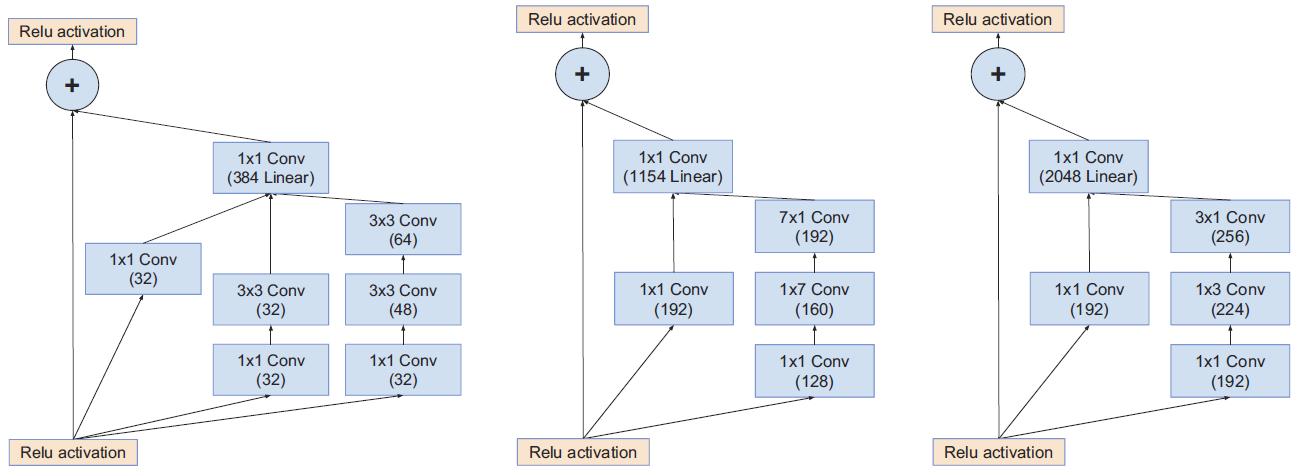
\includegraphics[width=\linewidth]{1_4.png}
        \caption{Inception-ResNet-v2}
    \end{figure}

    \begin{figure}
        \centering
        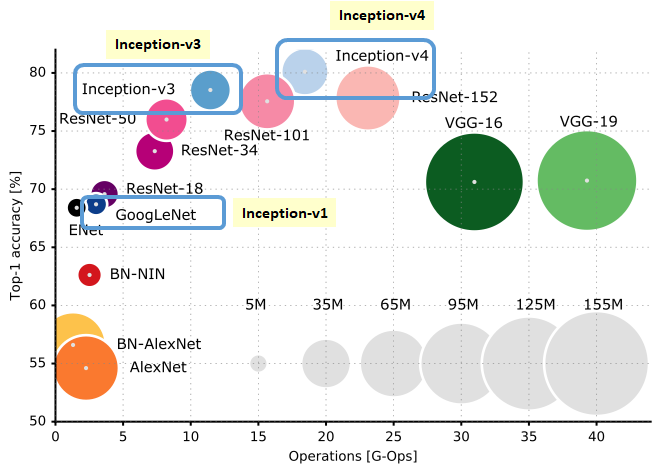
\includegraphics[width=0.8\linewidth]{1_5.png}
        \caption{Accuracy against Number of Operations}
    \end{figure}

\end{frame}

\begin{frame}[allowframebreaks]
    \frametitle{Object Detection}

    \begin{figure}
        \centering
        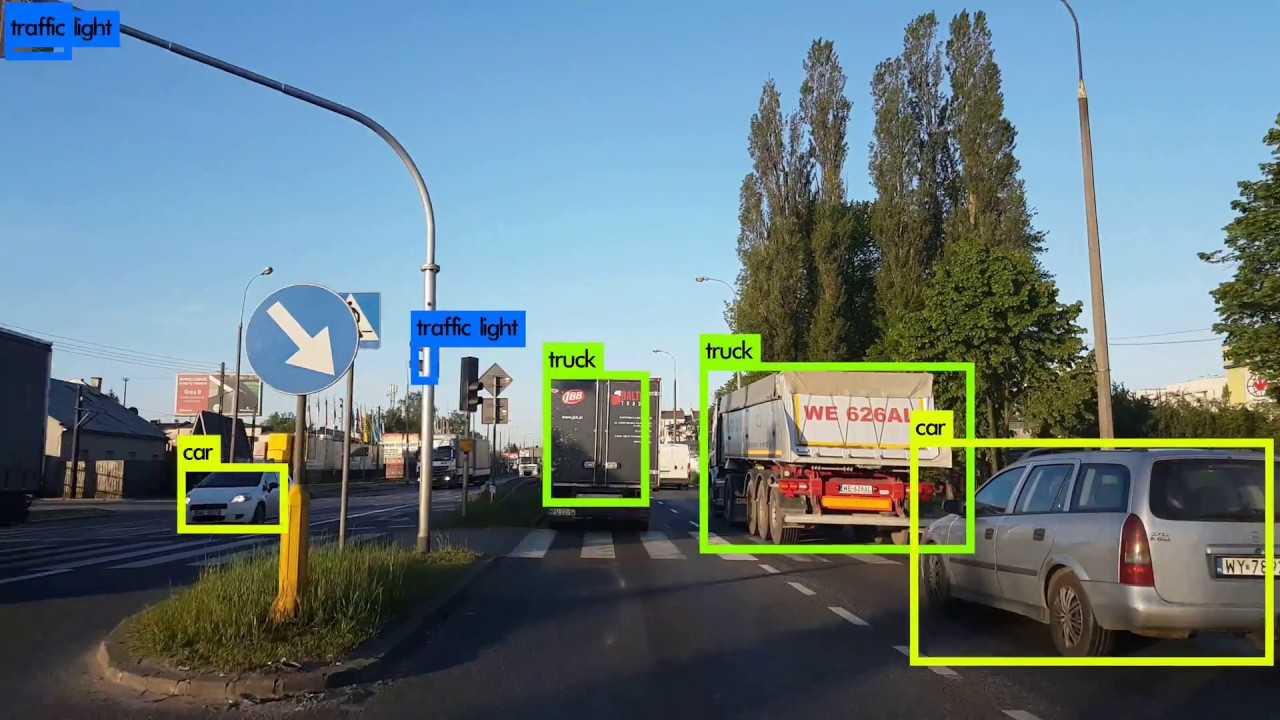
\includegraphics[width=0.95\linewidth]{2.jpg}
        \caption{}
    \end{figure}

    \begin{itemize}
        \item Region Proposals (R-CNN, Fast R-CNN, Faster R-CNN)
        \item Single Shot MultiBox Detector (SSD)
        \item You Only Look Once (YOLO)
    \end{itemize}

    \begin{figure}
        \centering
        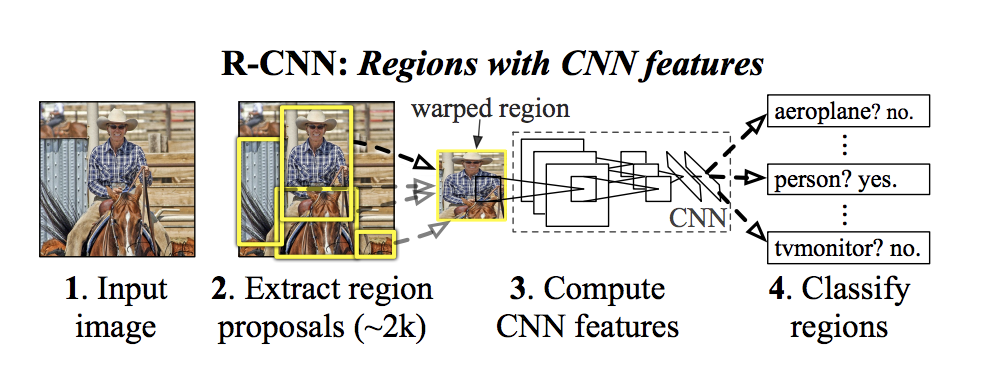
\includegraphics[width=0.99\linewidth]{2_2.png}
        \caption{R-CNN}
    \end{figure}

    \begin{figure}
        \centering
        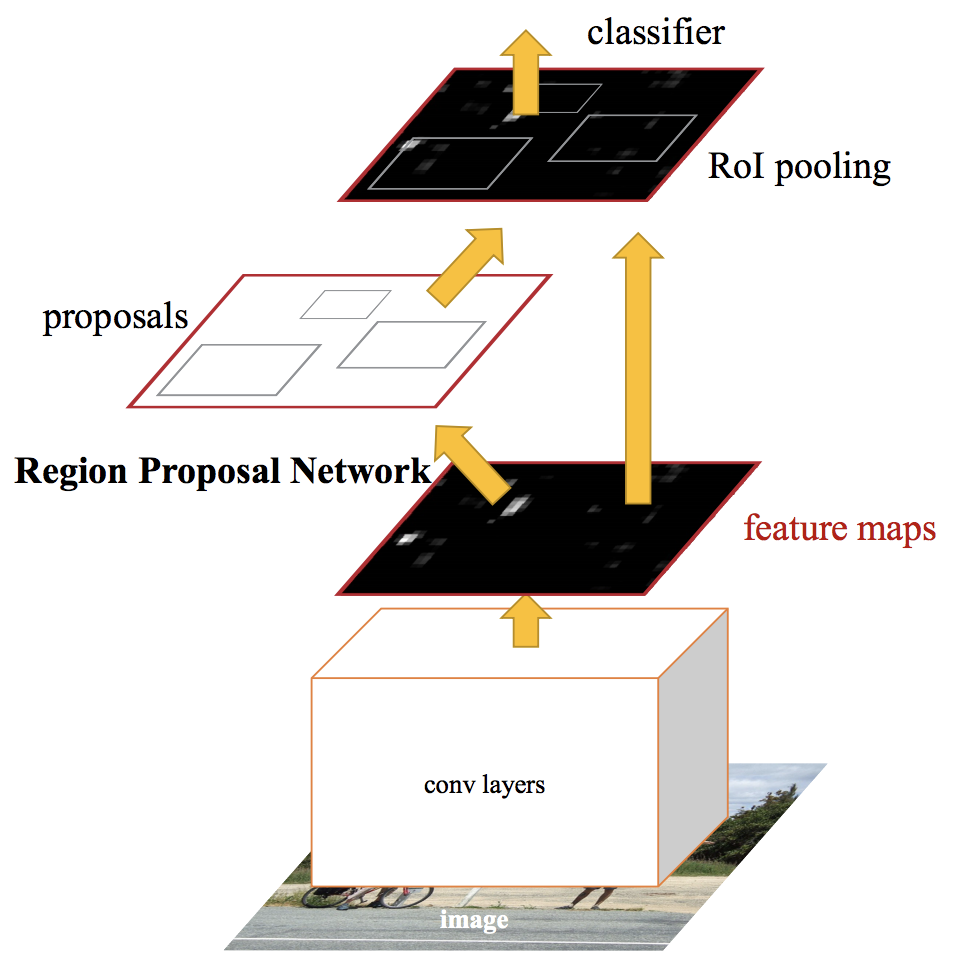
\includegraphics[width=0.6\linewidth]{2_1.png}
        \caption{Faster R-CNN}
    \end{figure}

    \begin{figure}
        \centering
        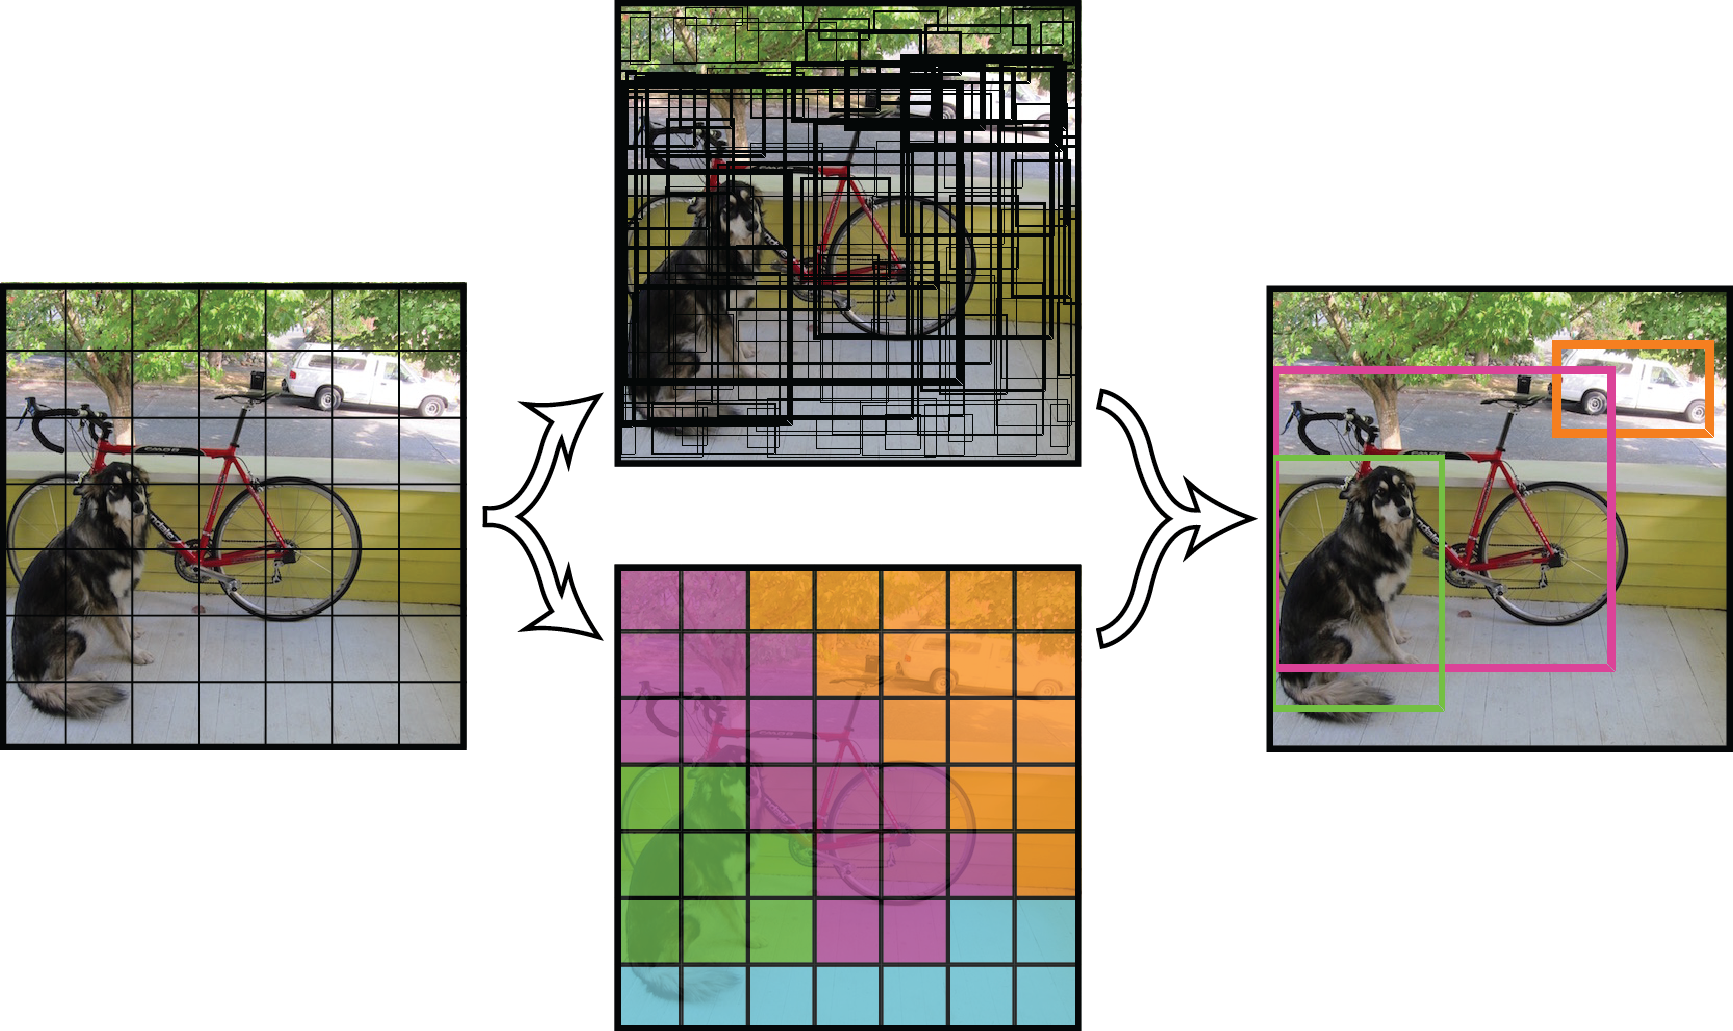
\includegraphics[width=0.9\linewidth]{2_3.png}
        \caption{You Only Look Once (YOLO)}
    \end{figure}

    \begin{figure}
        \centering
        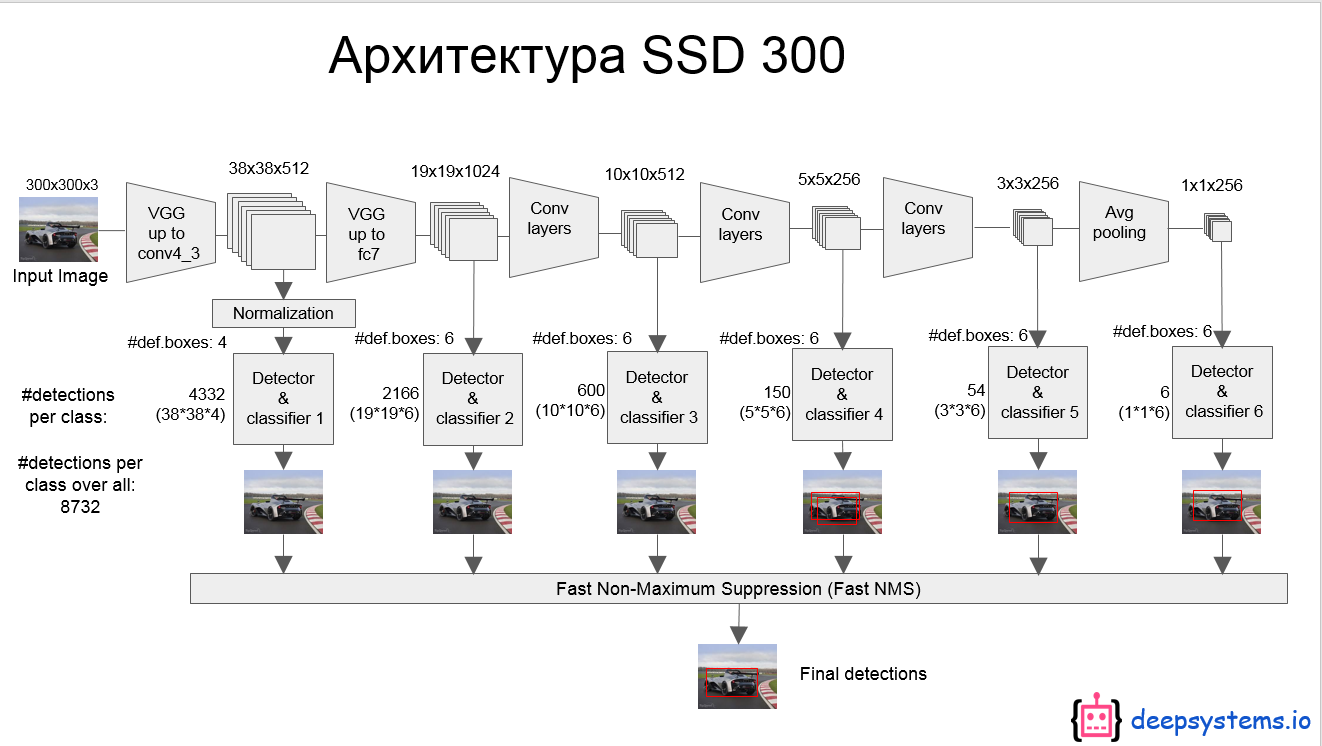
\includegraphics[width=\linewidth]{2_4.png}
        \caption{Single Shot MultiBox Detector (SSD)}
    \end{figure}

\end{frame}

\begin{frame}[allowframebreaks]
    \frametitle{Semantic Segmentation}

    \begin{figure}
        \centering
        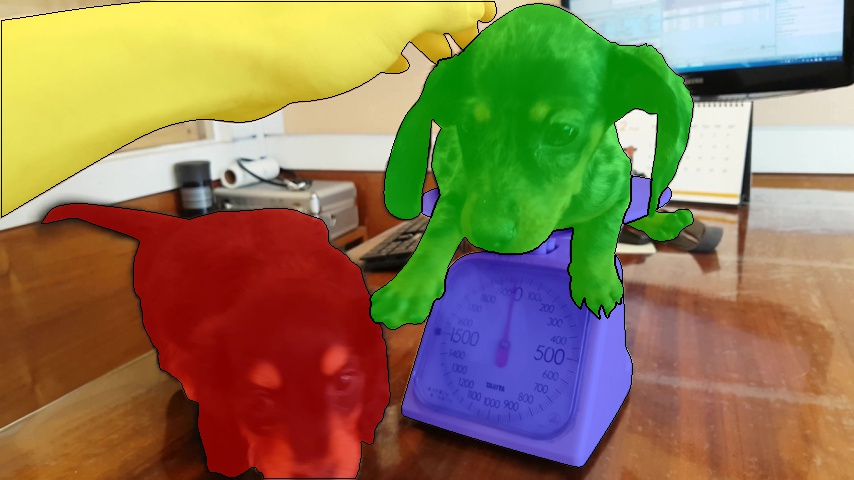
\includegraphics[width=0.95\linewidth]{3.jpg}
        \caption{}
    \end{figure}

    \begin{figure}
        \centering
        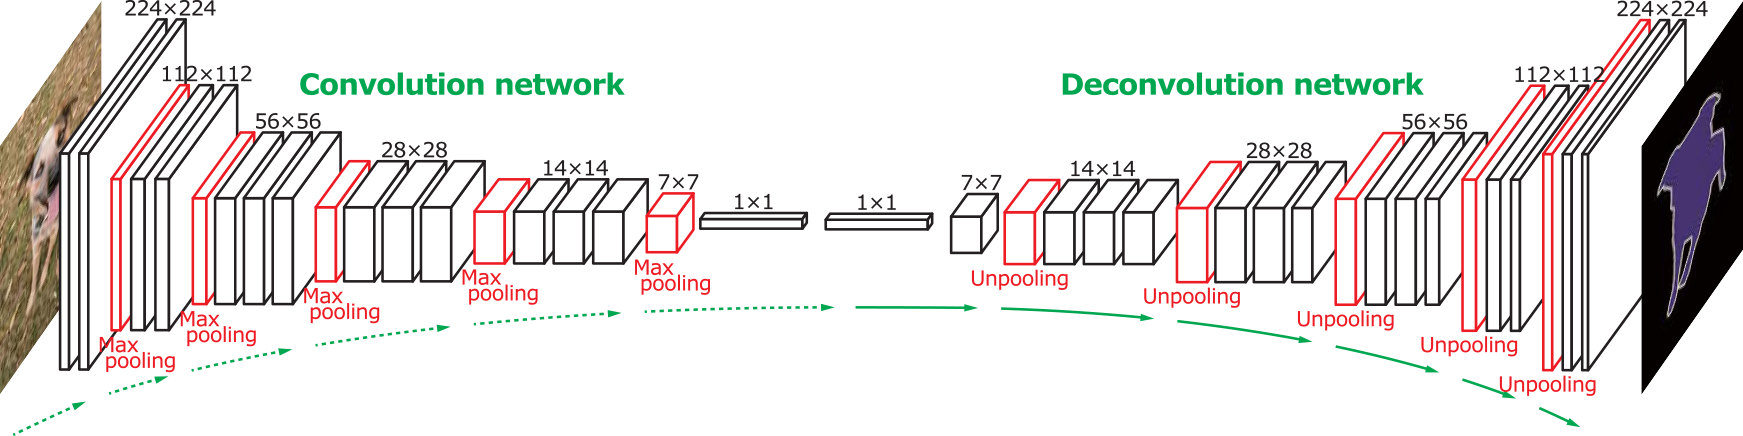
\includegraphics[width=0.95\linewidth]{3_1.png}
        \caption{Deconvolution Network}
    \end{figure}

    \begin{figure}
        \centering
        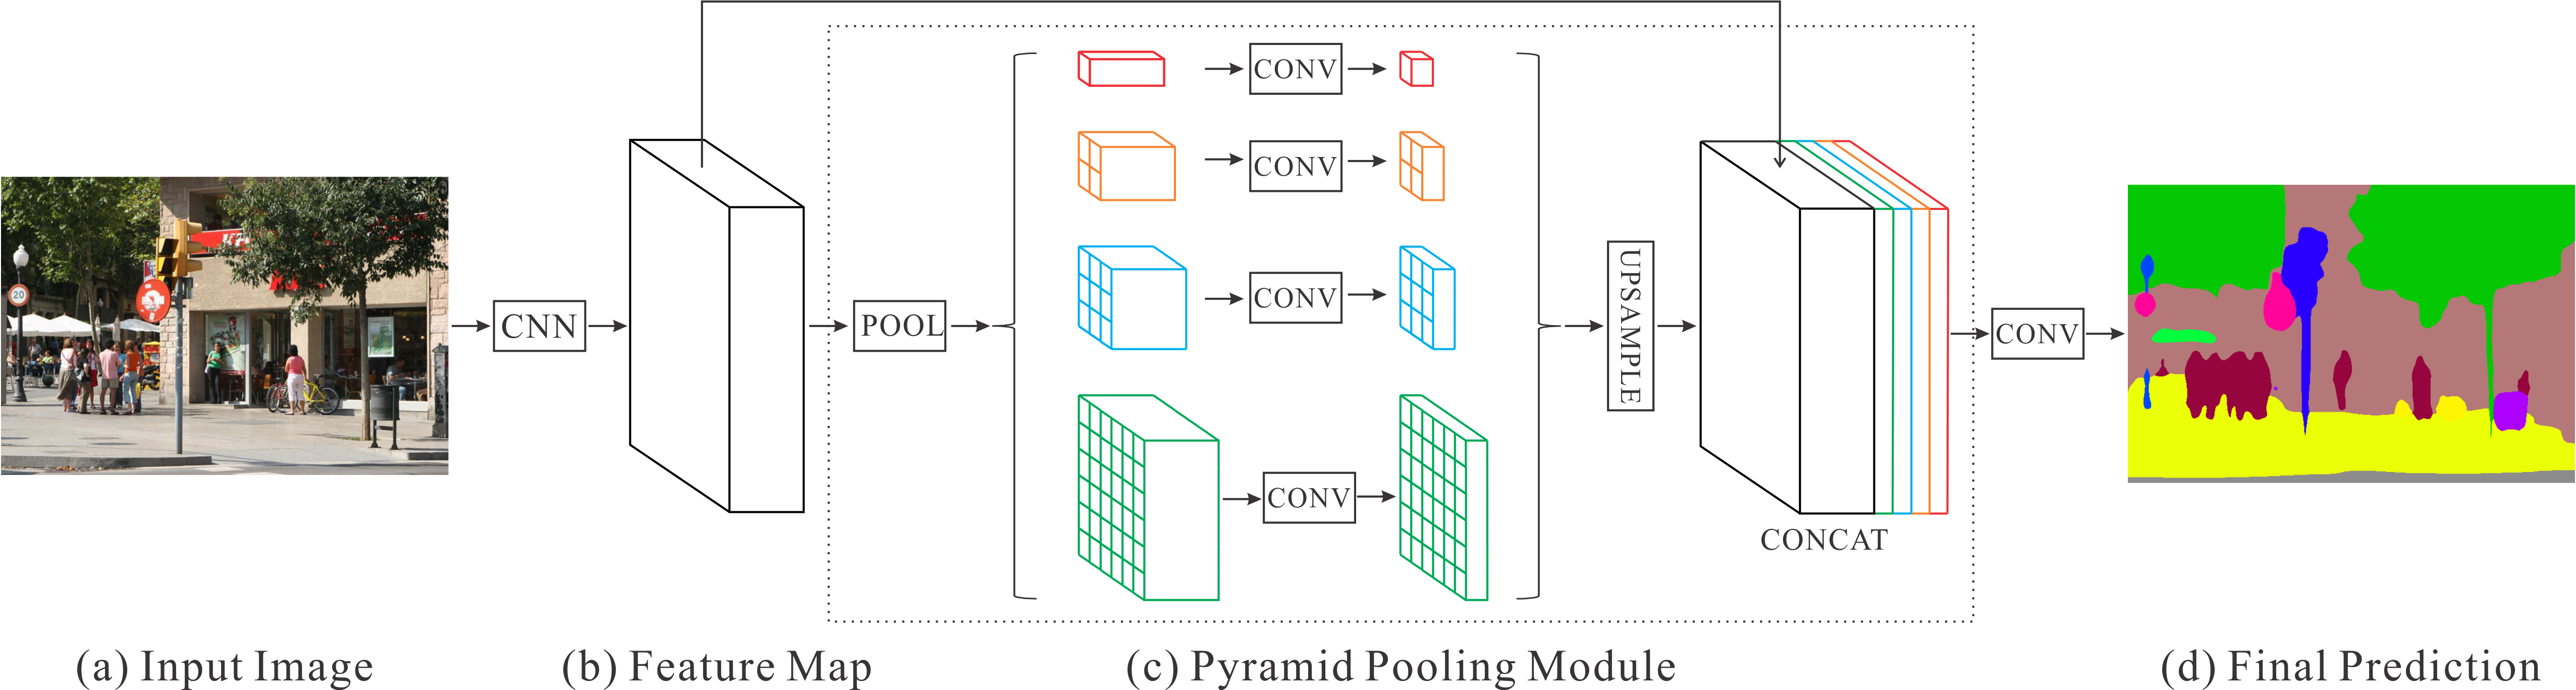
\includegraphics[width=0.95\linewidth]{3_2.png}
        \caption{Pyramid Scene Parsing Network}
    \end{figure}

\end{frame}

\begin{frame}
    \frametitle{Style Transfer}

    \begin{figure}
        \centering
        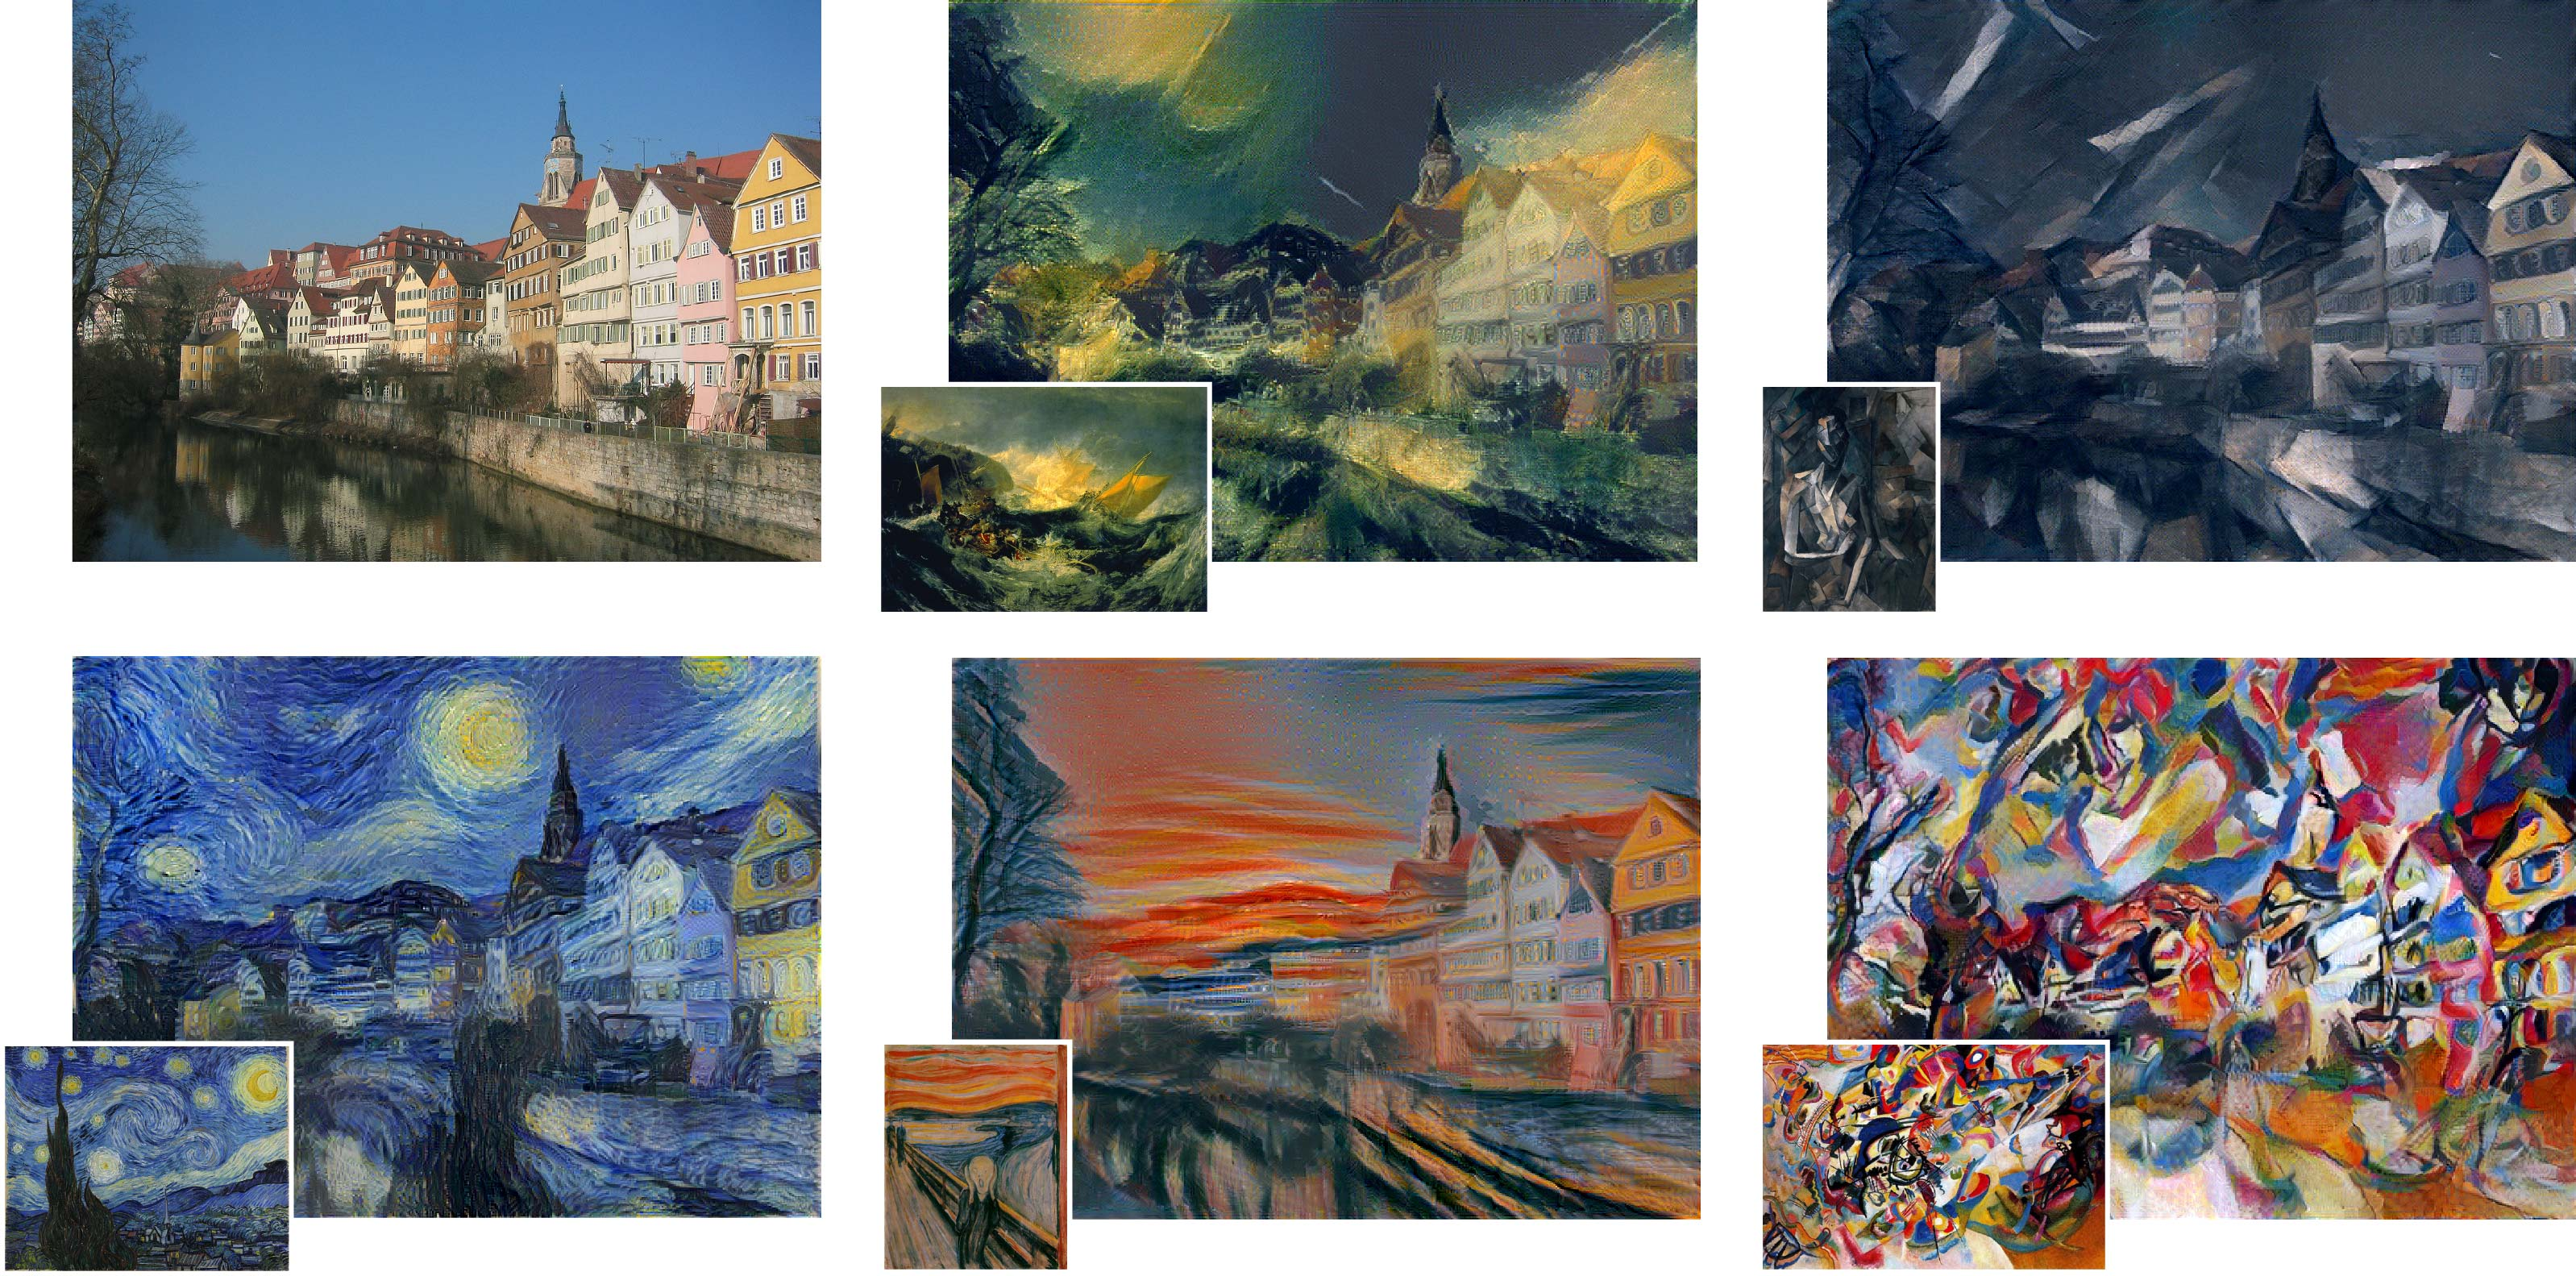
\includegraphics[width=0.95\linewidth]{4.jpg}
        \caption{}
    \end{figure}

\end{frame}

\begin{frame}
    \frametitle{Image Reconstruction}

    \begin{figure}
        \centering
        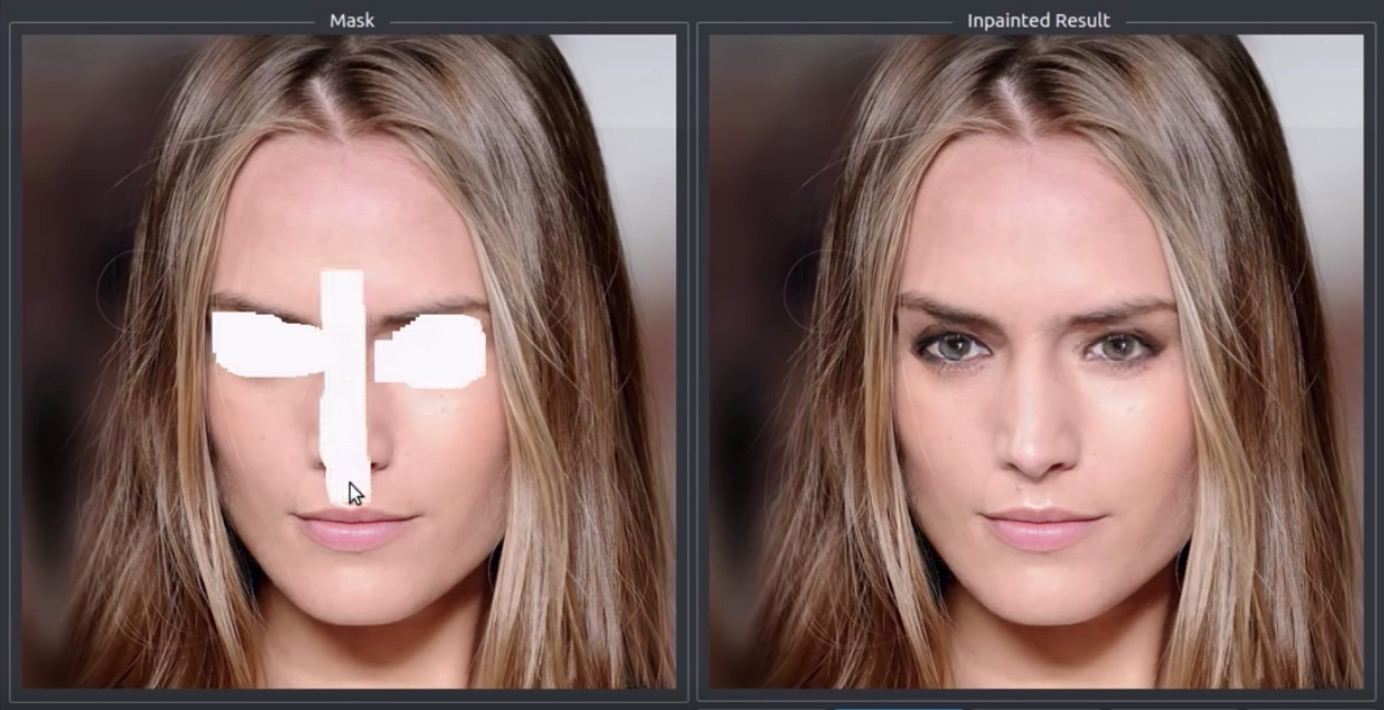
\includegraphics[width=0.95\linewidth]{5.jpg}
        \caption{}
    \end{figure}

\end{frame}

\begin{frame}[allowframebreaks]
    \frametitle{Image Colorization}

    \begin{figure}
        \centering
        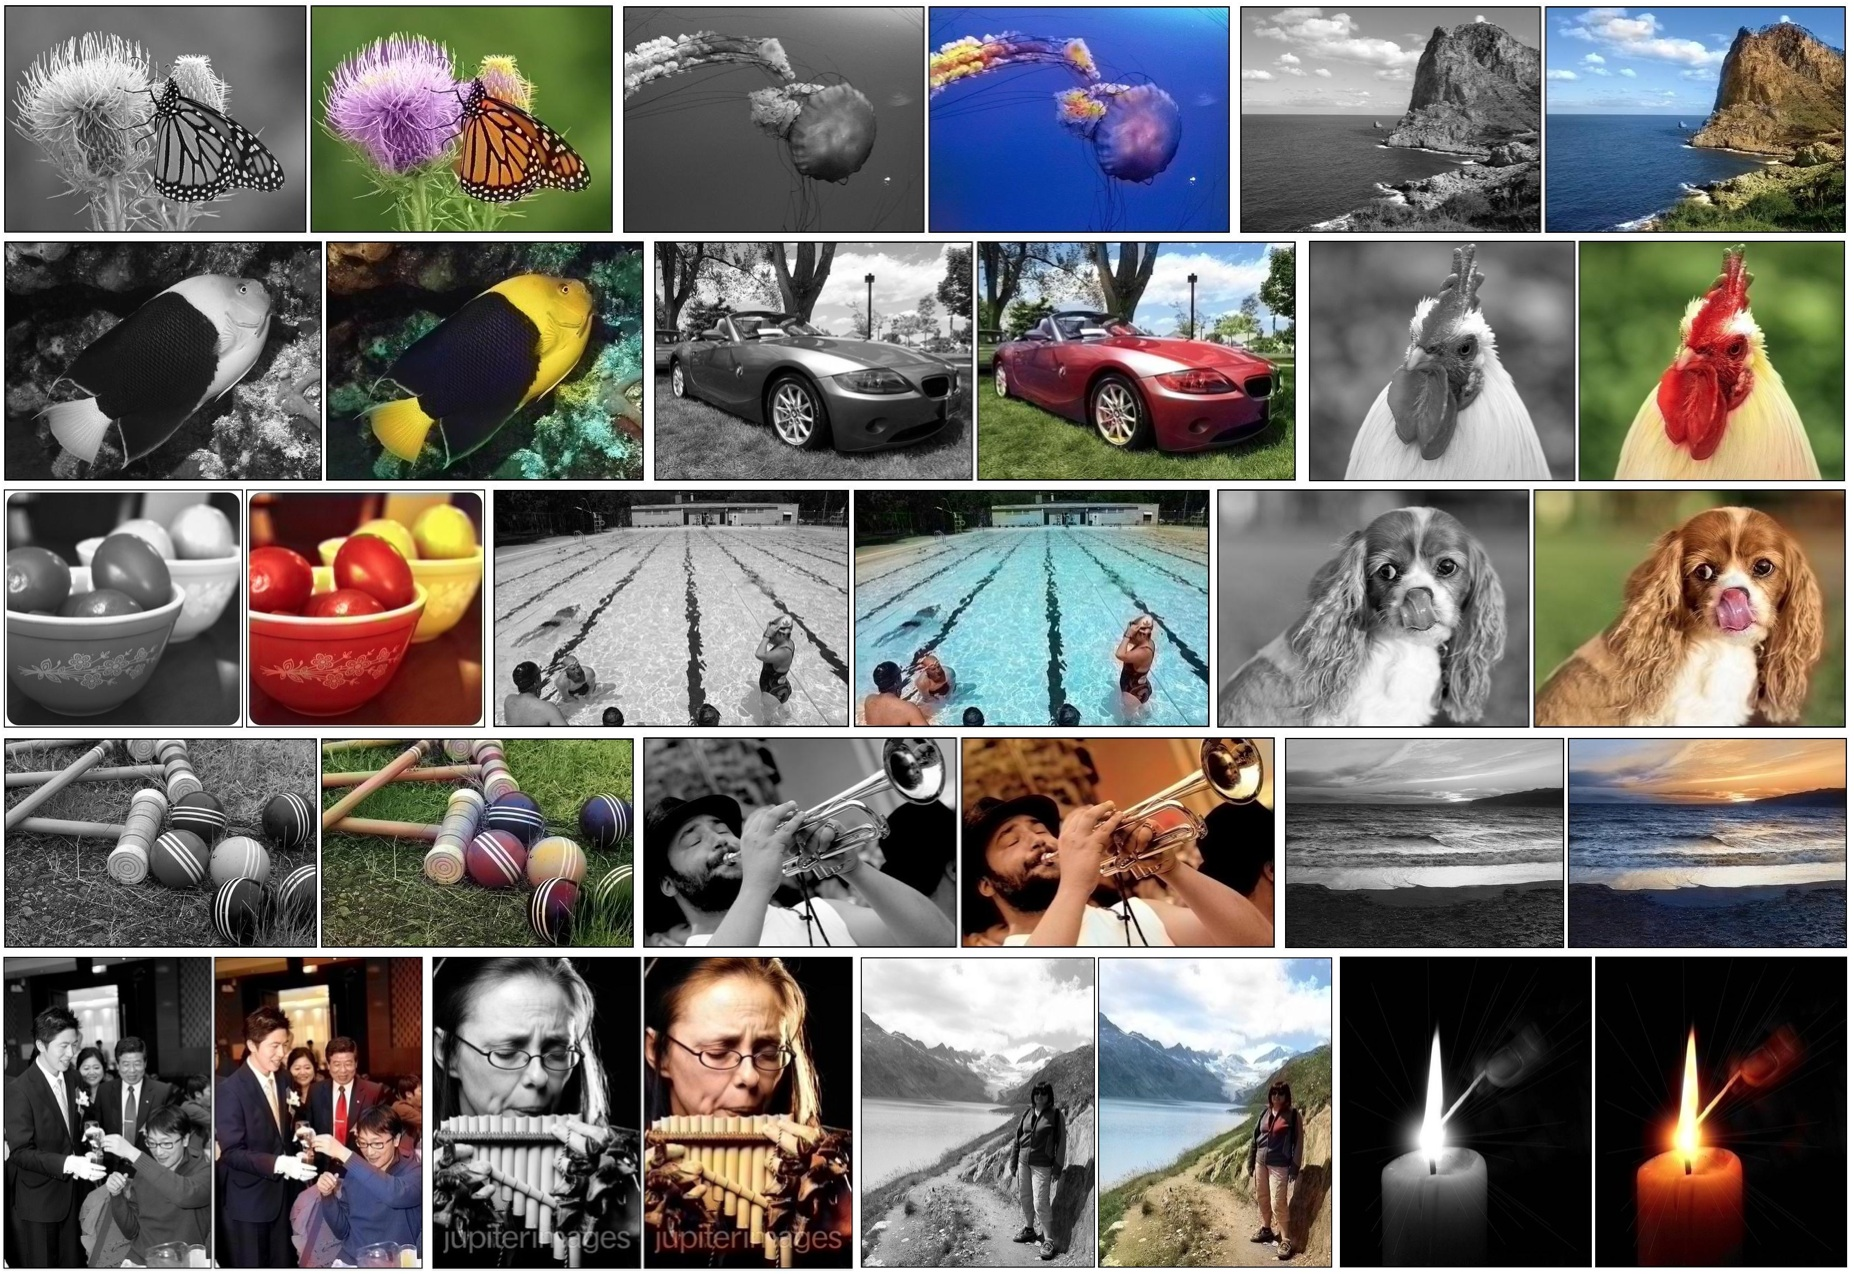
\includegraphics[width=0.95\linewidth]{6.jpg}
        \caption{}
    \end{figure}

    \begin{figure}
        \centering
        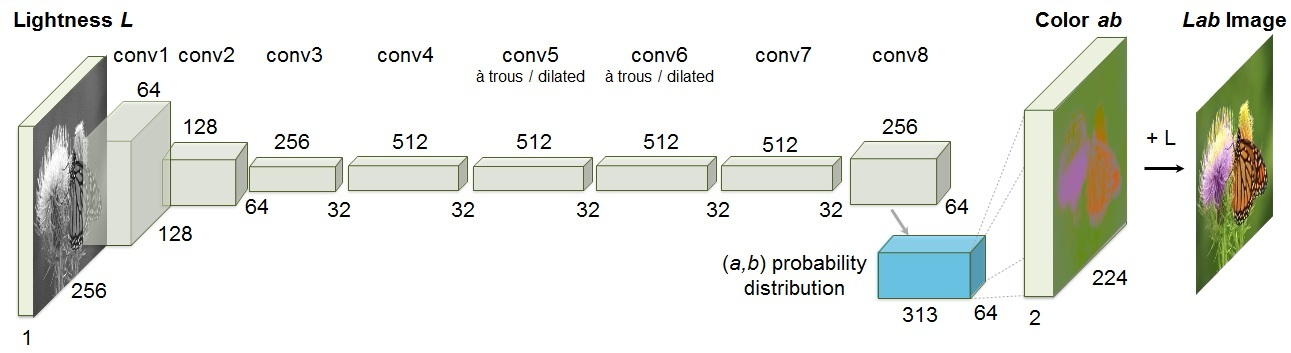
\includegraphics[width=0.95\linewidth]{6_1.jpg}
        \caption{}\cite{zhang2016colorful}
    \end{figure}

\end{frame}

\begin{frame}[allowframebreaks]
    \frametitle{Image Super-Resolution}

    \begin{figure}
        \centering
        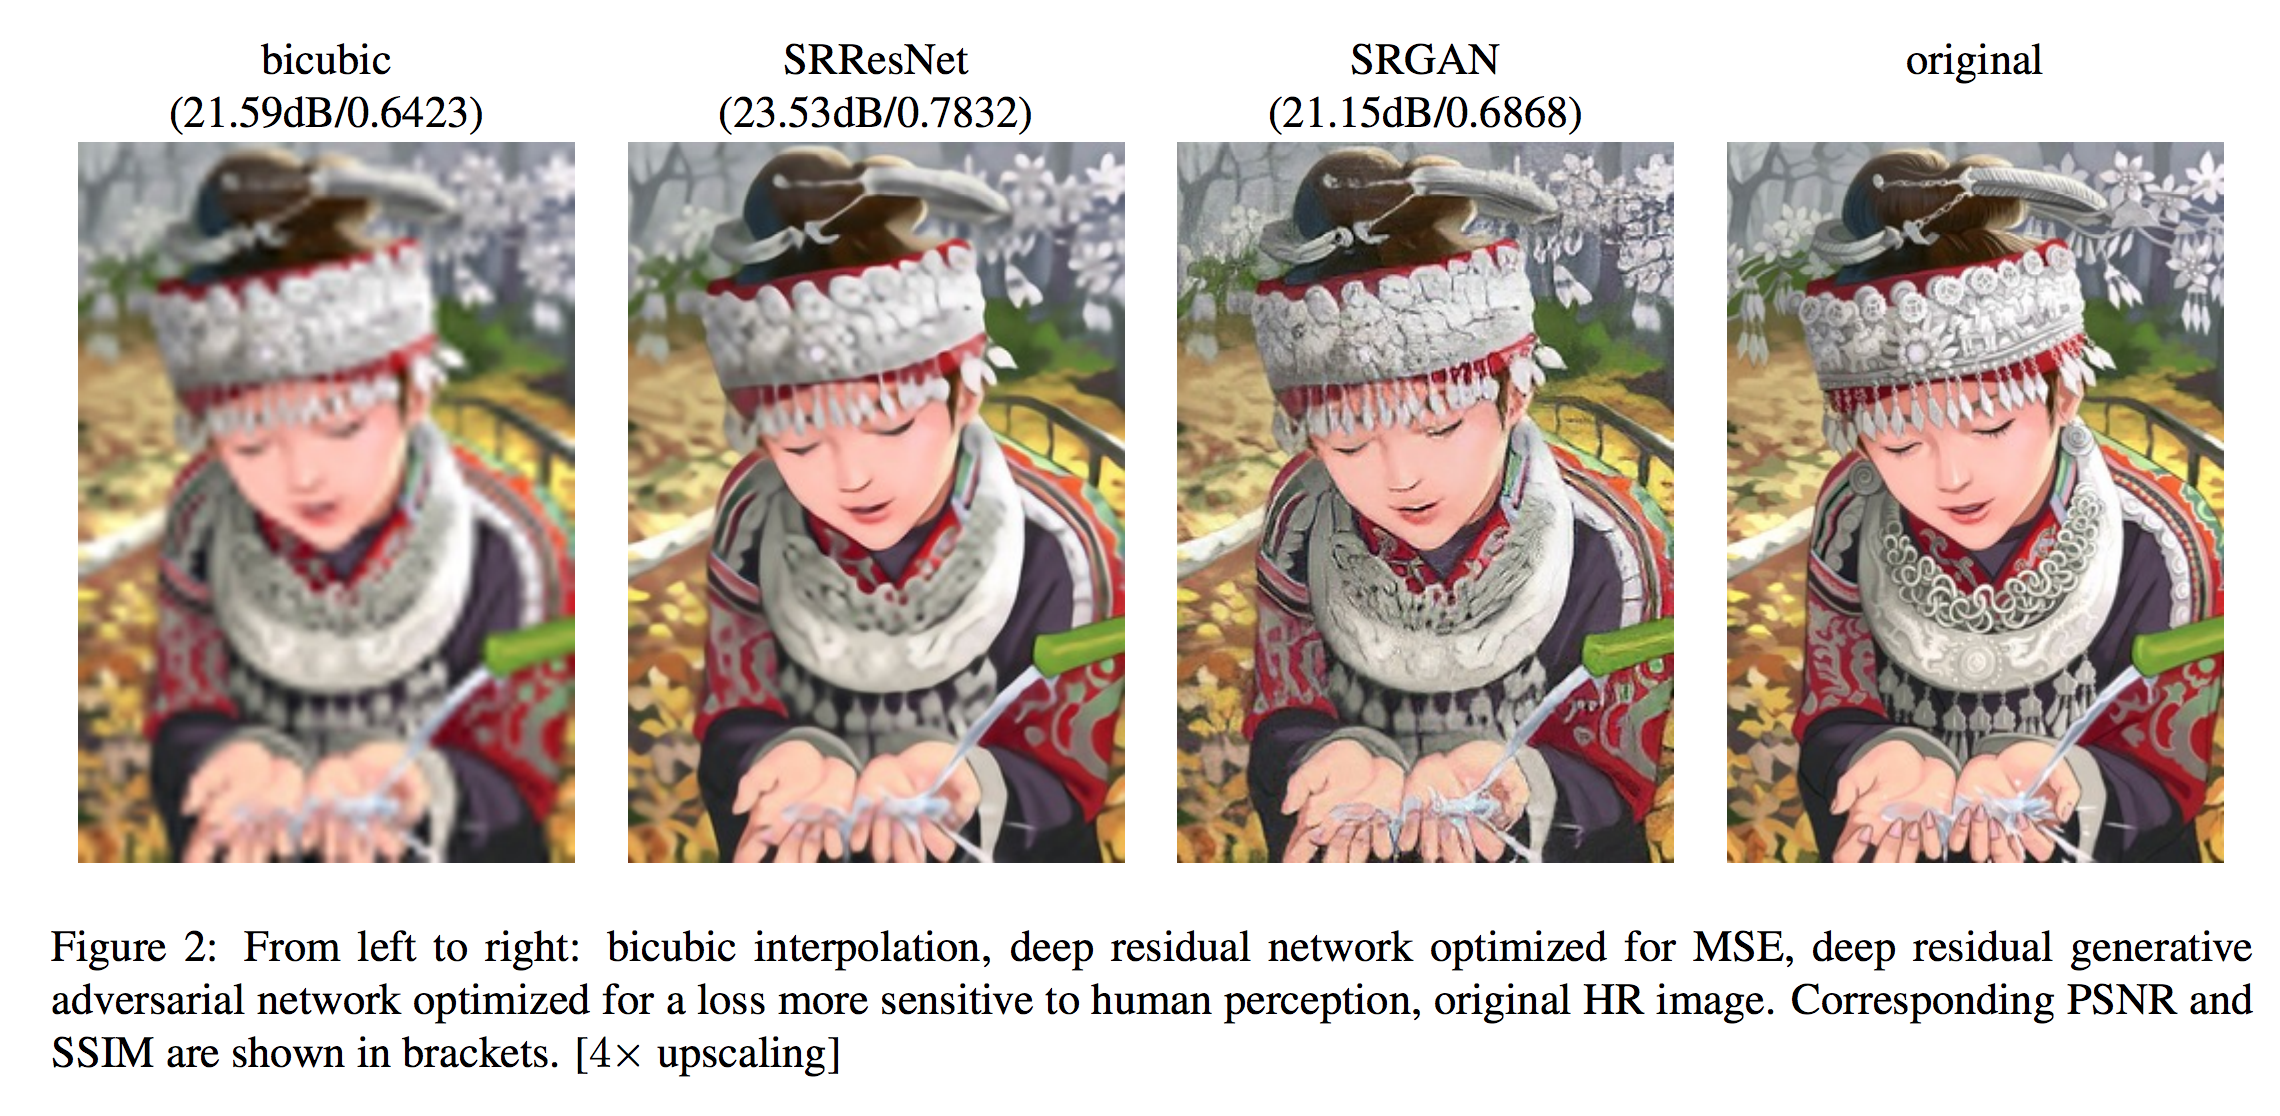
\includegraphics[width=0.95\linewidth]{7.png}
        \caption{}
    \end{figure}

    \begin{figure}
        \centering
        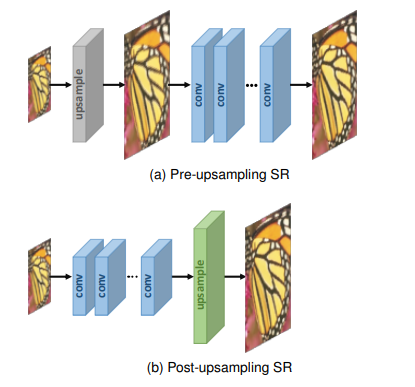
\includegraphics[width=0.6\linewidth]{7_1.png}
    \end{figure}

    \begin{figure}
        \centering
        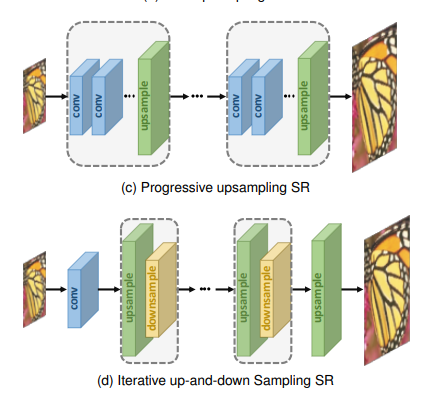
\includegraphics[width=0.6\linewidth]{7_2.png}
    \end{figure}

\end{frame}

\section{Natural Language Processing\cite{young2018recent}}

\begin{frame}[allowframebreaks]
    \frametitle{Word Embeddings}

    \begin{figure}
        \centering
        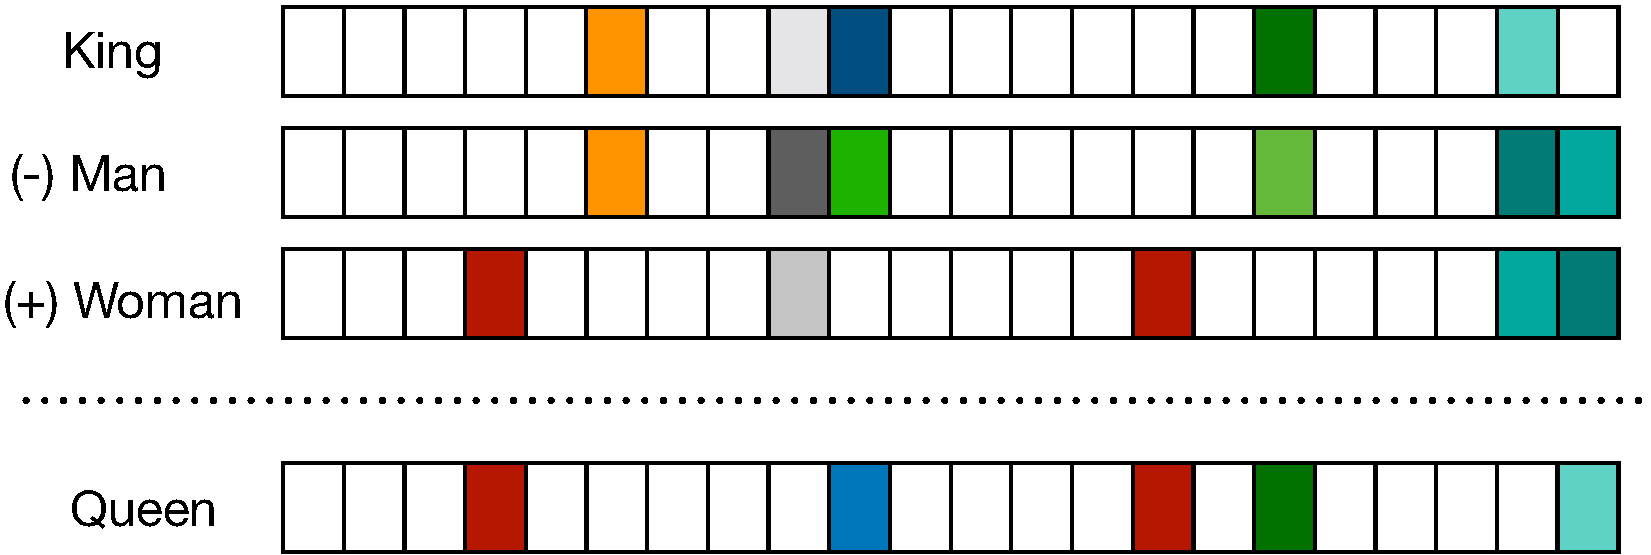
\includegraphics[width=\linewidth]{distributional.pdf}
        \caption{Distributional vectors represented by a ${\bf D}$-dimensional vector where ${\bf D} << {\bf V} $, where ${\bf V} $ is size of Vocabulary. }
    \end{figure}

    \begin{figure}
        \centering
        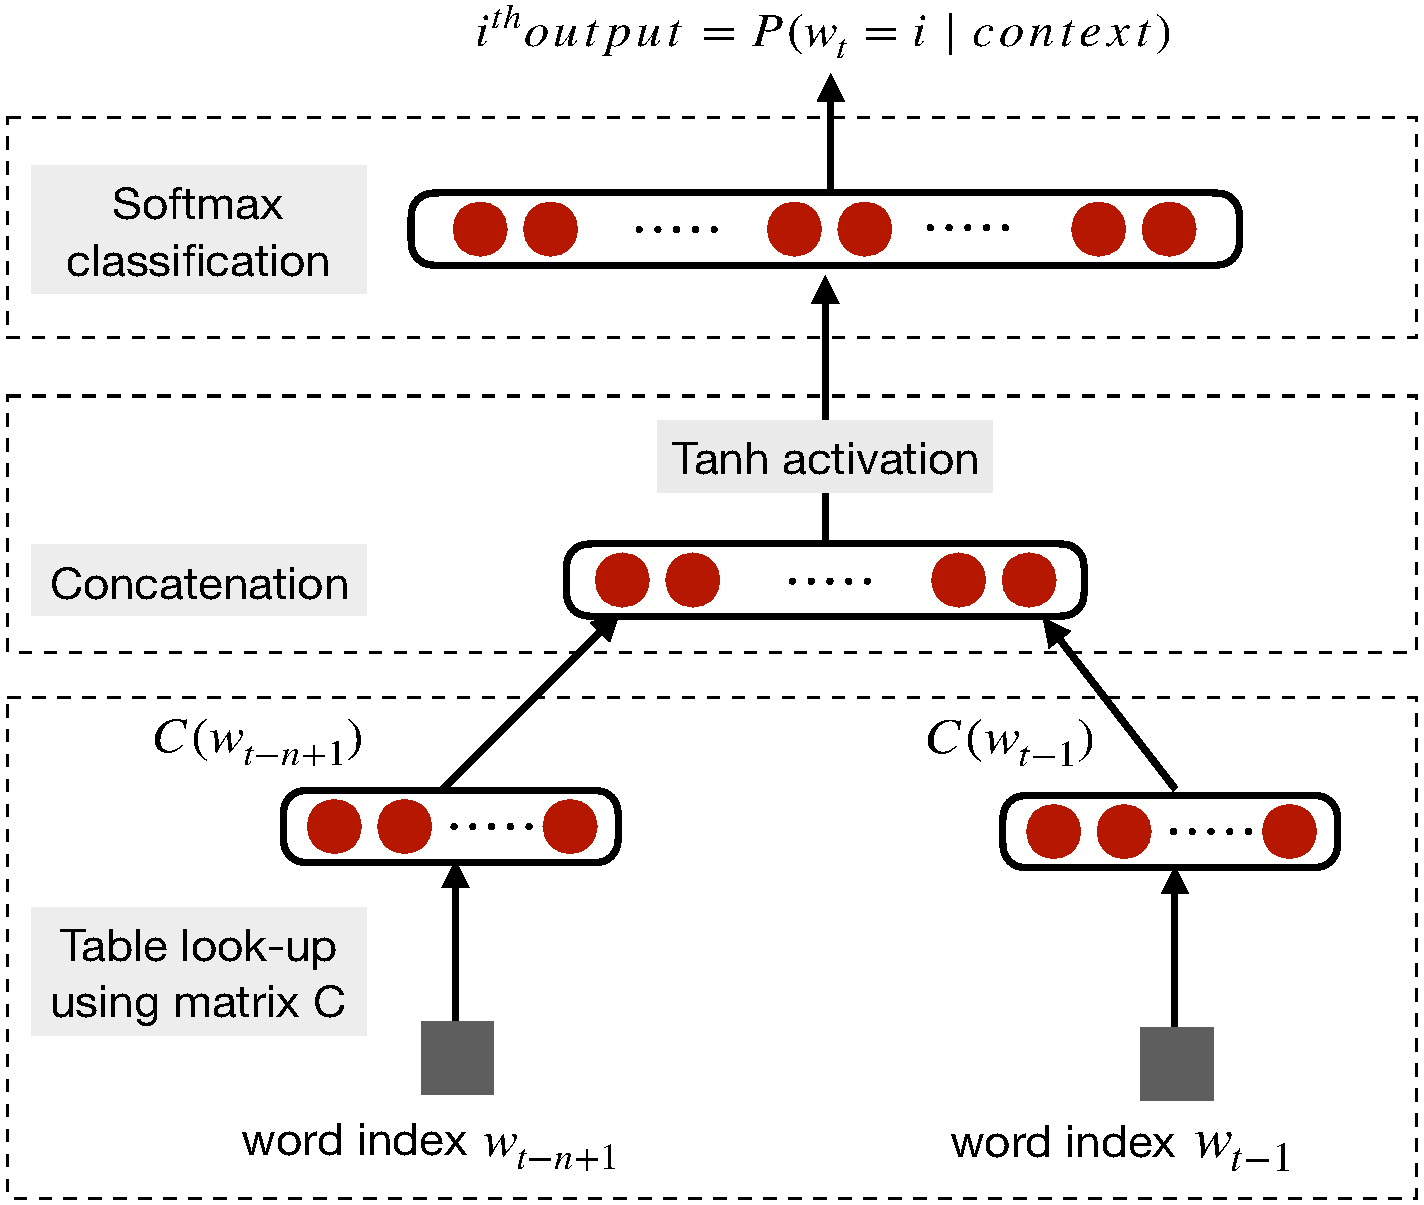
\includegraphics[width=.65\linewidth]{bengio.pdf}
        \caption{Neural Language Model. $C(i)$ is the $i^{th}$ word embedding.}
    \end{figure}
    
\end{frame}

% \begin{frame}[allowframebreaks]
%     \frametitle{Word2vec}

%     \begin{figure}
%         \centering
%         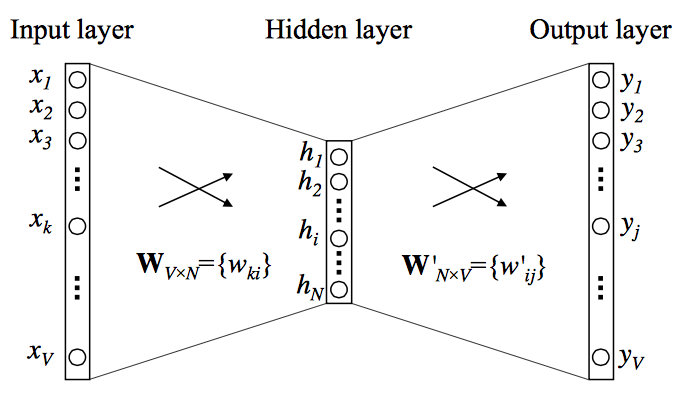
\includegraphics[width=\linewidth]{CBOW.png}
%         \caption{Model for CBOW}
%     \end{figure}

%     As shown in figure, the CBOW model is a simple fully connected neural network with one hidden layer. The input layer, which takes the one-hot vector of context word has ${V}$ neurons while the hidden layer has ${N}$ neurons. The output layer is softmax probability over all words in the vocabulary. The layers are connected by weight matrix 
%     ${\bf W} \in \mathcal{R}^{V \times N } $ and ${\bf W^{'}} \in \mathcal{R}^{H \times V}$, respectively. Each word from the vocabulary is finally represented as two learned vectors $ {\bf v_c} $ and ${\bf v_w}$, corresponding to context and target word representations, respectively. Thus, $k^{th}$ word in the vocabulary will have
%     \begin{gather}
%         {\bf v_c} = {\bf W_{(k,.)}} \quad and \quad {\bf v_w} = {\bf W^{'}_{(.,k)}}
%     \end{gather}

%     Overall, for any word $w_i$ with given context word $c$ as input, 
%     \begin{gather}
%         {p\left(\frac{w_i}{c}\right)} = {\bf y_i} = \frac{e^{u_i}}{\sum_{i=1}^{V} e^{u_i}} \quad where,\ \ {u_i} = {\bf v_{w_i}^T.v_c}
%     \end{gather}
%     The parameters $ {\bf \theta} = {\bf \{v_w, v_c\}}_{w,c \,\in\, \text{Vocab}}$ are learned by defining the objective function as the log-likelihood and finding its gradient as
%     \begin{gather}
%         {\bf l(\theta)} = {\bf \sum_{w \in Vocab} log\left(p\left(\frac{w}{c}\right)\right)} \\
%         {\bf \frac{\partial l(\theta)}{\partial v_w}} = {\bf v_c\left(1-p\left(\frac{w}{c}\right)\right)}
%     \end{gather}

%     In the general CBOW model, all the one-hot vectors of context words are taken as input simultaneously, i.e,
%     \begin{equation}
%         {\bf h} = {\bf W^T(x_1 + x_2 + ... + x_c)}
%     \end{equation}
    
% \end{frame}

\begin{frame}
    \frametitle{Convolutional Neural Networks}
    \begin{figure}
        \centering
        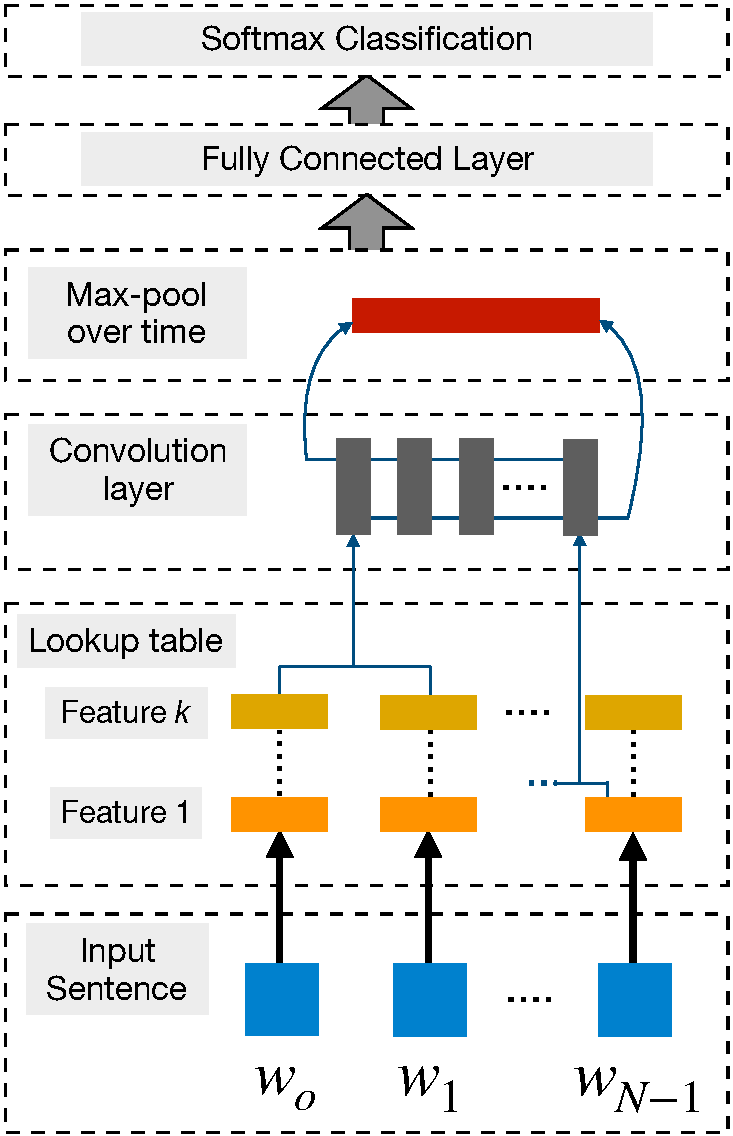
\includegraphics[width=0.4\linewidth]{collobertCNN.pdf}
    \end{figure}

\end{frame}

\begin{frame}
    \frametitle{Recurrent Neural Networks}
    
    \begin{figure}
        \centering
        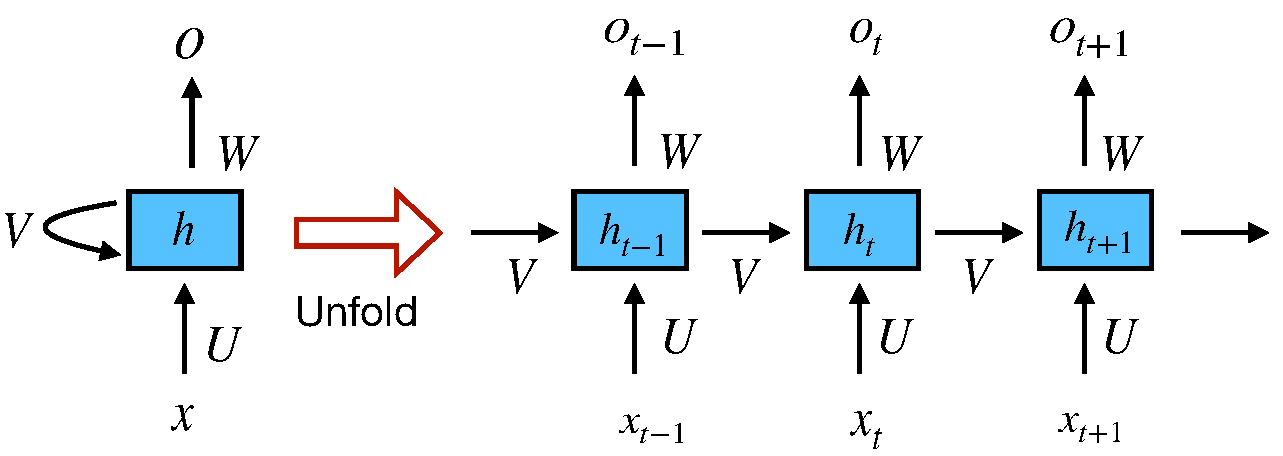
\includegraphics[width=\linewidth]{elmanrnn.pdf}
        \caption{Simple RNN}
    \end{figure}
\end{frame}

\begin{frame}
    \frametitle{Long Short-Term Memory}

    \begin{gather}
        {\bf x} = \left[ {\begin{array}{c}
            \bm{h}_{t-1}\\
            \bm{x}_t \\
            \end{array} } \right]\\
        f_t = \sigma(W_f . {\bf x} + b_f)\\
        i_t = \sigma(W_i . {\bf x} + b_i) \\
        o_t = \sigma(W_o . {\bf x} + b_o)\\
        c_t = f_t \odot c_{t-1} + i_t \odot tanh(W_c . X + b_c) \\
        h_t = o_t \odot tanh(c_t)
    \end{gather}

\end{frame}

\begin{frame}
    \frametitle{Gated Recurrent Units}

    \begin{gather}
        {\bf z} = \sigma(U_z . {\bf x_t} + W_z . {\bf h_{t-1}})\\
        {\bf r} = \sigma(U_r . {\bf x_t} + W_r . {\bf h_{t-1}})\\
        {\bf s_t} = tanh(U_z . {\bf x_t} + W_s .( h_{t-1} \odot {\bf r}) )\\
        {\bf h_t} = (1 - {\bf z}) \odot {\bf s_t} + {\bf z} \odot {\bf h_{t-1}} 
    \end{gather}

\end{frame}

\begin{frame}
    \frametitle{}

    \begin{figure}
        \centering
        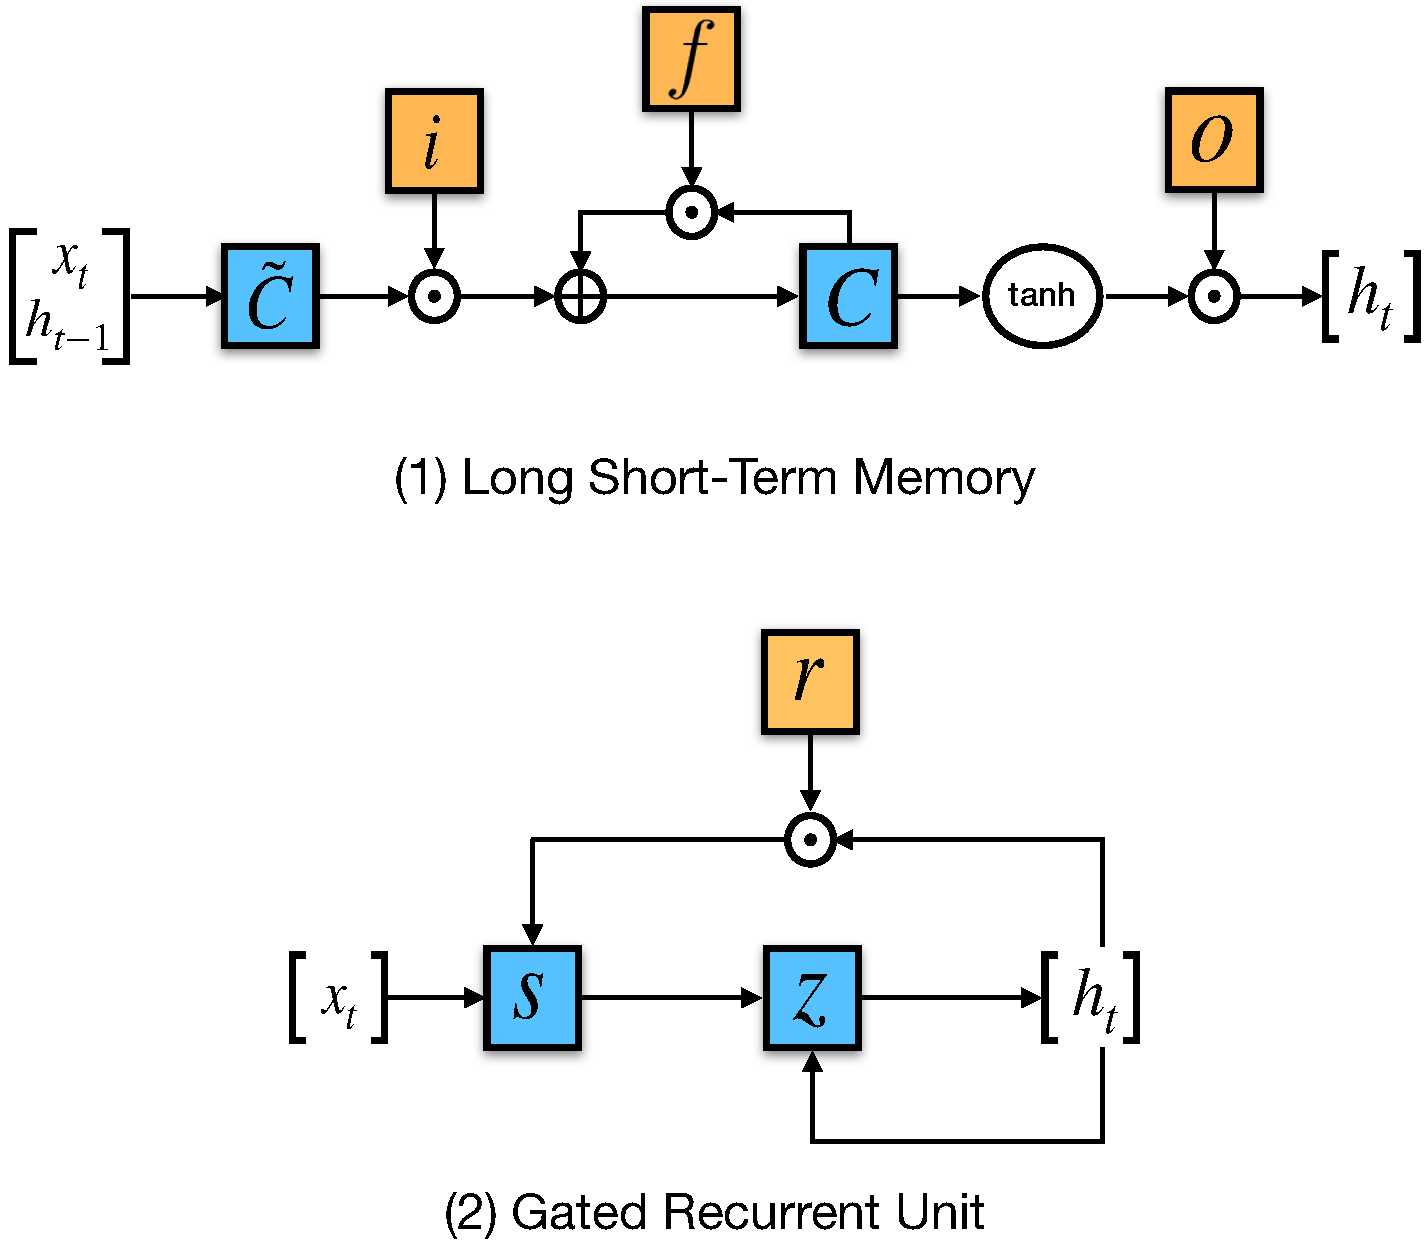
\includegraphics[width=.7\linewidth]{LSTMGRU.pdf}
        \caption{Simple RNN}
    \end{figure}

\end{frame}

\section{other}

\begin{frame}
    \frametitle{Visual Question Answering}
    \begin{figure}
        \centering
        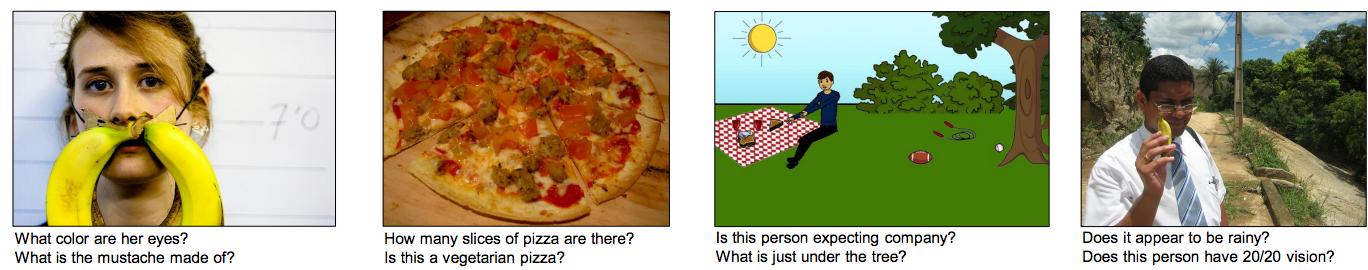
\includegraphics[width=\linewidth]{vqa.jpg}
    \end{figure}
\end{frame}

\begin{frame}
    \frametitle{Deep Q-Learning}
    \begin{figure}
        \centering
        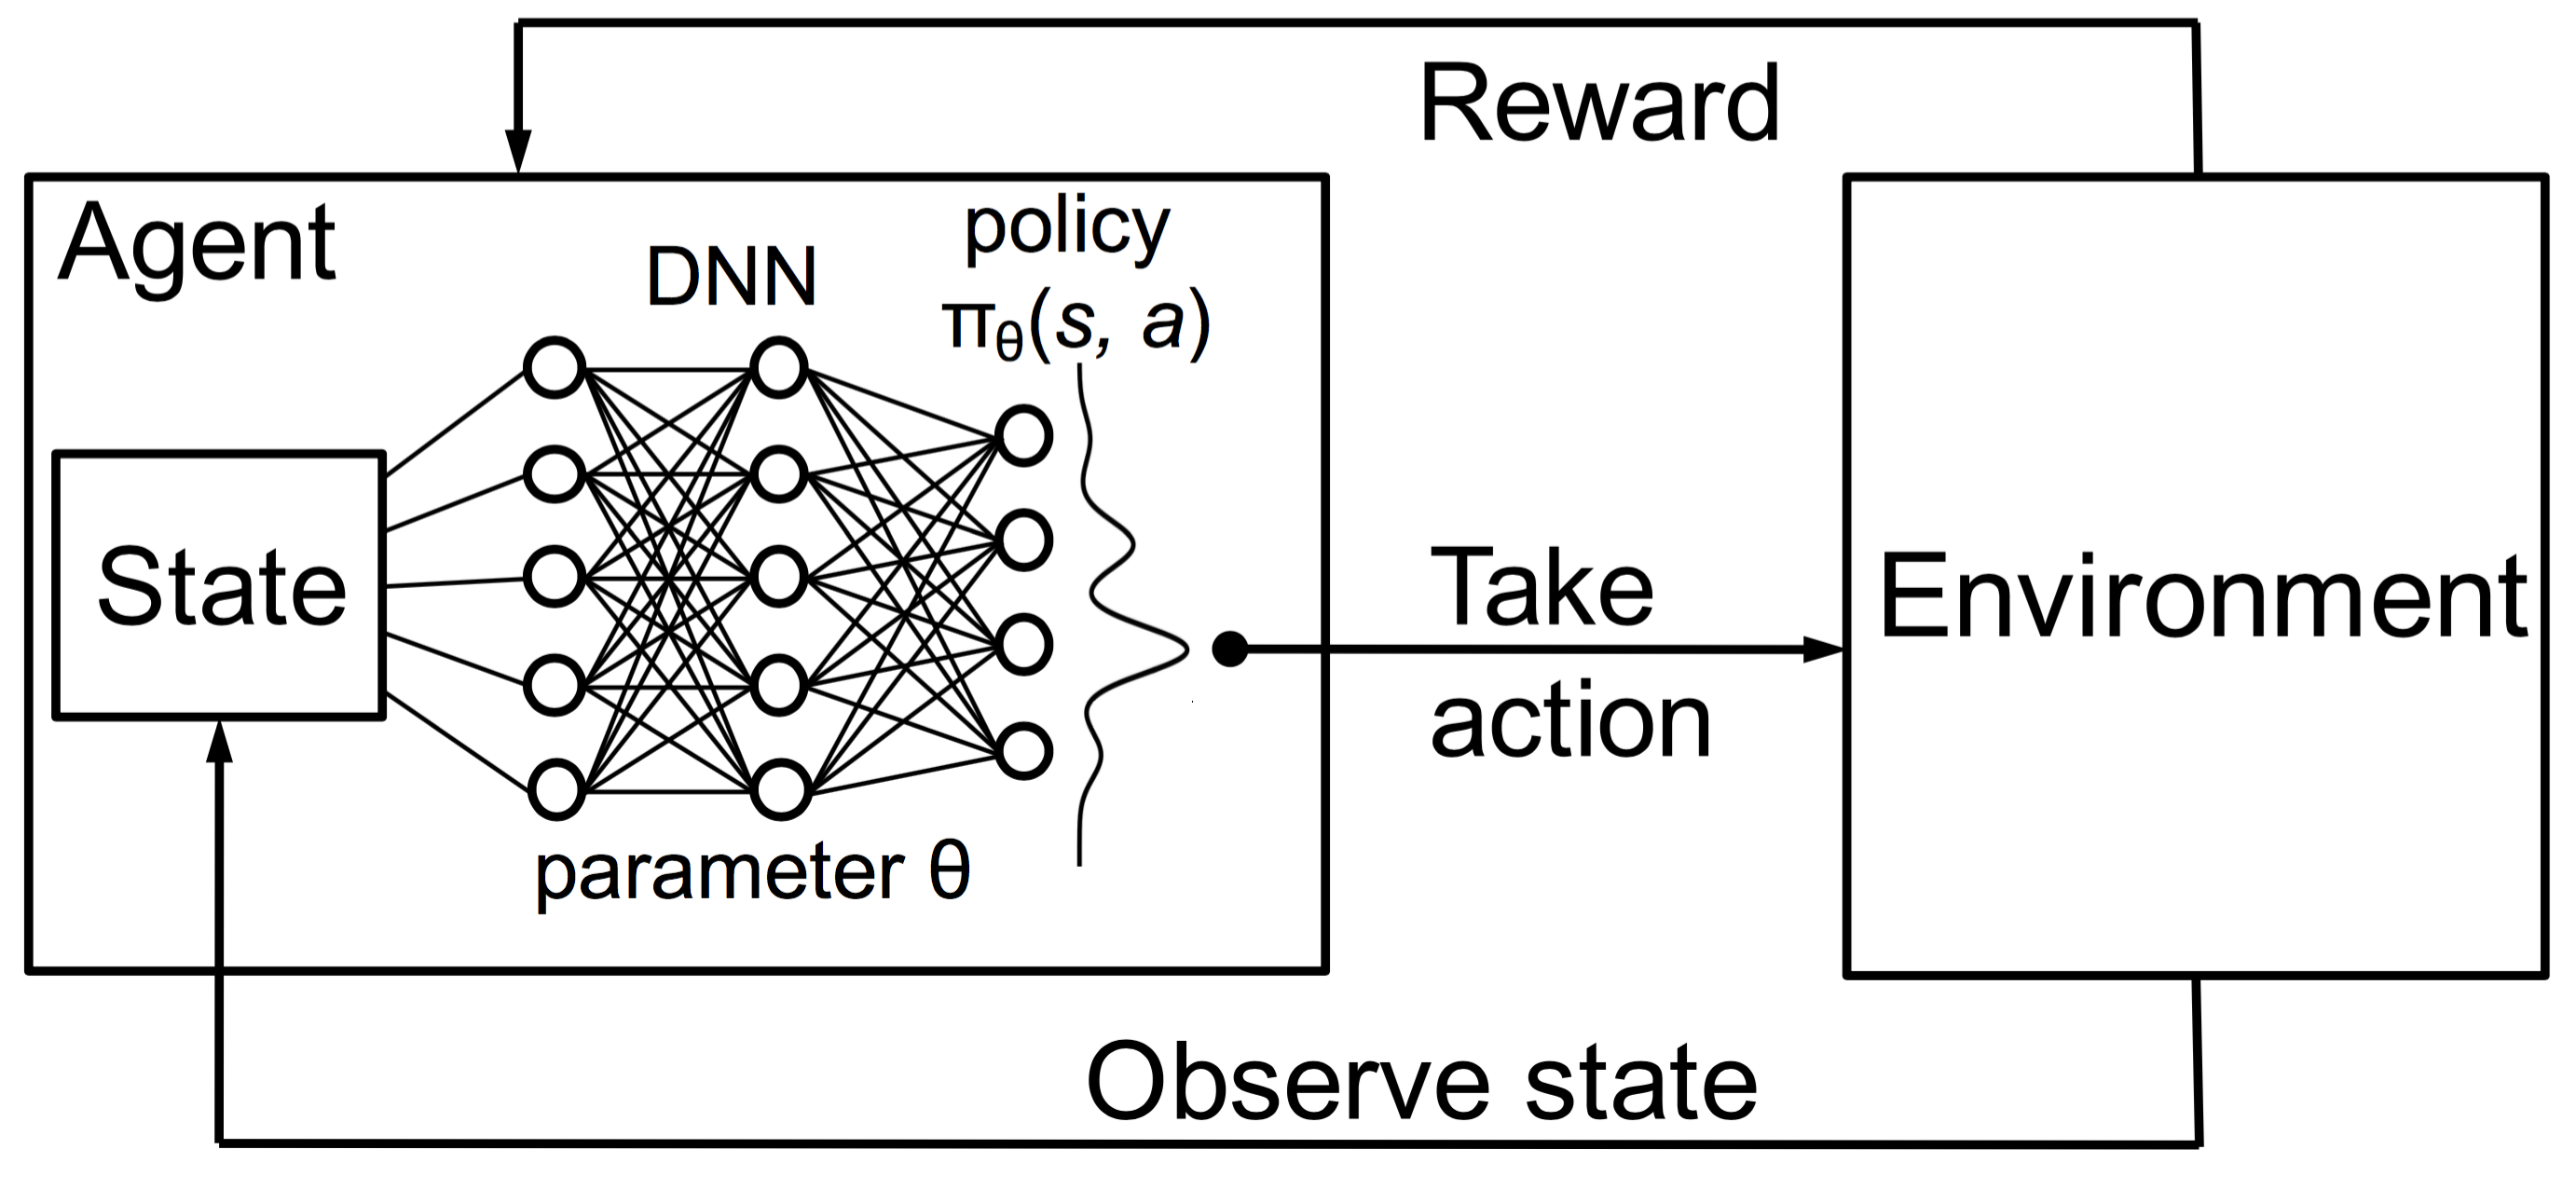
\includegraphics[width=\linewidth]{dql.png}
    \end{figure}
\end{frame}

\begin{frame}[standout]
    Questions
\end{frame}

\begin{frame}[allowframebreaks]
    \frametitle{Reference}

    \bibliographystyle{plain}
    \bibliography{cite}

\end{frame}

\end{document}

